%!TEX root = ../trajectory-grouping.tex
Zur Berechnung der \GrpStruktur müssen wir gemäß \cref{def:grpstrukur} den reduzierten Reeb-Graphen und die maximalen Gruppen berechnen.
Dazu berechnen wir zunächst den unreduzierten Reeb-Graphen $\mathcal{R}$ und dann die maximalen Gruppen.
Mit diesen Informationen ist die Reduktion von $\mathcal{R}$ ein trivialer Nachbearbeitungsschritt.

Für die Berechnung des Reeb-Graphen ist eine Datenstruktur zur dynamischen Speicherung von Bäumen nötig.
Eine solche verwaltet einen Wald von Bäumen mit disjunkten Knotenmengen und unterstützt dabei eine Reihe von Operationen auf diesen Bäumen.
Die Operationen, die wir benötigen, sind in \cref{tbl:operationenST} aufgeführt.
\begin{table}[p]
	\Centering
	\caption{Operationen, die von ST-Bäumen unterstützt werden (nach \cite{parsaReeb})}\label{tbl:operationenST}
	\begin{tabular}{lp{.7\textwidth}}
		\toprule
		$\mathtt{parent}(x)$ & Gibt den Eltern-Knoten von $x$ zurück, falls dieser existiert; \texttt{null}, falls $x$ ein Wurzelknoten ist.\\
		$\mathtt{root}(x)$ & Gibt die Wurzel des Baumes zurück, zu dem $x$ gehört.\\
		$\mathtt{link}(x_1,x_2,w)$ & Verbindet verschiedene Bäume durch das Einfügen einer Kante zwischen $x_1$ und $x_2$, der das Gewicht $w$ zugeordnet wird.\\
		$\mathtt{cut}(x_1,x_2)$ & Entfernt die Kante zwischen $x_1$ und $x_2$ und trennt damit einen Baum in zwei auf.\\
		$\mathtt{minWeight}(x)$ & Gibt einen Knoten auf dem Pfad von $x$ zur Wurzel zurück, der minimales Gewicht zu seinem Elternknoten hat; \texttt{null}, falls $x$ ein Wurzelknoten ist.\\
		$\mathtt{evert}(x)$ & Macht $x$ zur Wurzel des Baumes, zu dem $x$ gehört.\\
		\bottomrule
	\end{tabular}
\end{table}
Eine Datenstruktur, die alle diese Operationen in $\mathcal{O}(\log n)$ Zeit, wobei $n$ die Gesamtzahl der Knoten ist, realisiert, ist unter anderem ein \Index{ST-Baum} nach \textcite{dynamictrees}.
Das im Folgenden geschilderte Vorgehen von \textcite{buchin2015} zur Berechnung des Reeb-Graphen $\mathcal{R}$ basiert auf einem Algorithmus von \textcite{parsaReeb}, der diese ST-Bäume benutzt.

\begin{figure}[hbt]
	\Centering
	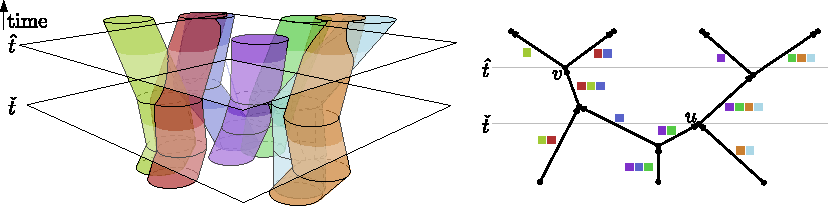
\includegraphics[width=.9\textwidth]{Bilder/manifold.pdf}
\end{figure}

\section{Berechnung des Reeb-Graphen} % (fold)
\label{sec:berechnung_reeb}
Wir wollen den Reeb-Graphen $\mathcal{R}$ des dreidimensionalen Raumes $\mathcal{M}$ aus \cref{sec:trajek_reeb} bezüglich der Höhenfunktion berechnen -- die \enquote{Höhe} ist hier aber die Zeit!
Folglich ist es natürlich, die Berechnung mittels eines Sweep-Algorithmus zu realisieren.
Unsere Sweep-Ebene ist also die $xy$-Ebene, die $\mathcal{M}$ von unten nach oben -- also chronologisch -- überstreicht.

In \cref{sec:background_reeb} über die differentialtopologischen Hintergründe haben wir bereits gesehen, dass sich der Reeb-Graph nur an den kritischen Werten verändert.\footnote{unter der Annahme, dass $\mathcal{M}$ eine glatte Mannigfaltigkeit ist, sodass kritische Werte überhaupt definiert sind}
Dies ermöglicht uns die notwendige Diskretisierung des Sweeps: Ein Knoten im Reeb-Graph kann nur auftreten, wenn zwei Komponenten verschmelzen (Merge), eine Komponente zerteilt wird (Split) oder eine Komponente beginnt oder endet, was alles notwendigerweise dadurch verursacht wird, dass zwei Entitäten direkt zusammenhängend werden (\emph{Connect}-Ereignis) oder es nicht länger sind (\emph{Disconnect}-Ereignis).\footnote{oder, dass das Ende des Beobachtungszeitraumes erreicht ist}
Definieren wir unsere Queue bzw. $z$-Struktur also als die Folge aller Zeitpunkte zu denen zwei Entitäten genau den Abstand $2 \varepsilon$ haben, so enthält die Queue auf jeden Fall alle Zeitpunkte, an denen $\mathcal{R}$ aktualisiert werden muss.

Tatsächlich filtern wir schon bei der Berechnung dieser Queue Zeitpunkte heraus, die nicht \enquote{kritisch} sein können, das heißt die keine kritischen Werte sind.
Außerdem teilen wir die Zeitpunkte in diesem Arbeitsschritt bereits in \emph{Connect}- und \emph{Disconnect}-Ereignisse auf.
Wie dies genau vonstatten geht und wie die Queue konkret gespeichert wird, wird in \cref{sub:berechnung_queue} erläutert.
In \cref{sub:xy_struktur} wird dann die für einen Sweep-Algorithmus außerdem benötigte $xy$-Struktur beschrieben, bevor in \cref{sub:behandlung_der_ereignisse} die Verarbeitung der Ereignisse aus der Queue inklusive der Initialisierung der $xy$-Struktur behandelt wird.
Um später die maximalen Gruppen berechnen zu können, wird jede Kante in $\mathcal{R}$ noch mit der zugehörigen Komponente beschriftet.

\subsection{Berechnung der Queue} % (fold)
\label{sub:berechnung_queue}
Gegeben Entitäten $x$ und $y$ wollen wir eine Liste $L_{xy}$ aller Ereignisse berechnen, die diese beiden Entitäten betreffen.
Diese soll chronologisch sortiert sein und nur echt verschiedene Zeitpunkte enthalten.
Weiter sollen sich \emph{Connect}- und \emph{Disconnect}-Ereignisse stets abwechseln, was dazu dient, für den Reeb-Graphen uninteressante Ereignisse herauszufiltern wie zum Beispiel den Fall, dass der Abstand von $x$ und $y$ nur bis auf exakt $2 \varepsilon$ sinkt und danach wieder steigt.

Dazu betrachten wir in zeitlicher Reihenfolge die $\tau$ Zeitintervalle.
In einem solchen $\benbrace*{t_u,t_{u+1}}$ bewegen sich $x$ und $y$ nur entlang je einer Geraden, sodass der Abstand eine konvexe Funktion beschreibt.
Insbesondere gibt es entweder $k$ mit $k \in \set*{0,1,2}$ Zeitpunkte aus $\benbrace*{t_u,t_{u+1}}$, an denen der Abstand genau $2 \varepsilon$ ist oder dies gilt für jeden Zeitpunkt $t \in \benbrace*{t_u,t_{u+1}}$.
Es lässt sich in $\mathcal{O}(1)$ Zeit bestimmen, welcher der Fälle eintritt, und welches ggf. die $k$ Zeitpunkte sind.
Im ersten Fall fügen wir die $k$ Zeitpunkte in die Liste ein, im zweiten nur die Randpunkte $t_u$ und $t_{u+1}$; in beiden Fällen fügen wir die Zeitpunkte nicht ein, falls dadurch die Eindeutigkeit verletzt werden würde (asymptotisch kein zusätzlicher Aufwand, da nur das zuletzt eingefügte Element betrachtet werden muss).

In einem zweiten Schritt bereinigen wir $L_{xy}$ nun wie folgt: Wir iterieren über $L_{xy}$ und berechnen dabei für jeden Eintrag $t_i$, ob $x$ und $y$ im offenen Intervall $(t_i,t_{i+1})$ direkt zusammenhängend sind (Abstand beim Mittelpunkt bestimmen).
Finden wir dadurch Zeitpunkte in $L_{xy}$, an denen sich der Zusammenhang von $x$ und $y$ nicht ändert, so entfernen wir diese aus der $L_{x,y}$.\footnote{Dies kann passieren, wenn ein solcher Zeitpunkt mit einem der Zeitstempel der Trajektorien übereinstimmt}
Die Verbleibenden beschriften wir entsprechend mit \emph{Connect} oder \emph{Disconnect}.
Auf das Bereinigen kann man verzichten, dann müssen während des Sweeps aber mehr Sonderfälle betrachtet werden.

$L_{xy}$ besteht aus $\mathcal{O}(\tau)$ Zeitpunkten und alle obigen Berechnungen kosten zusammen $\Theta(\tau)$ Zeit.
Berechnen wir diese Listen für alle $x,y$ und vereinigen sie unter Benutzung eines Min-Heaps\footnote{ein \emph{direct $k$-way merge}: die minimalen Elemente aller Listen werden in einem Min-Heap verwaltet, um in das kleinste in logarithmischer Zeit finden zu können} zu einer Liste $L$, so entstehen also insgesamt $\mathcal{O}(\tau n^2 \log n^2) = \mathcal{O}(\tau n^2 \log n)$ Kosten und $L$ enthält $\mathcal{O}(\tau n^2)$ Zeitpunkte.
Beim Zusammenführen der Listen $L_{xy}$ speichern wir zu jedem \emph{Connect}-Ereignis einen Zeiger auf das nächste \emph{Disconnect}-Ereignis der gleichen Entitäten, sofern dies existiert.
Falls dies nicht existiert, soll der Zeiger auf $t_\tau$, also das Ende des betrachteten Zeitraumes, zeigen.
Dies ist asymptotisch betrachtet kein zusätzlicher Aufwand.
Diese Zeiger sind wichtig, um gewisse Kantengewichte effizient -- das heißt in höchstens $\mathcal{O}(\log n)$ -- berechnen zu können (siehe Methode $\textsc{Insert}(x,y)$ in \cref{alg:funktionen}).

Anmerkung: Dieses Verfahren ist einigermaßen komplex, sorgt aber dafür, dass während des Sweeps keine Sonderfälle betrachtet werden müssen. 
Alternativ könnte man auch Listen für alle Paare von Entitäten für jeden der $\tau$ Zeitabschnitte betrachten und diese einfach konkatenieren, was offensichtlich auch $\mathcal{O}(\tau n^2 \log n^2)$ Zeit kostet.
Das Problem dabei ist aber, dass man auch dabei nicht ohne Weiteres\footnote{wie zB. das Verwalten des \enquote{letzten} Ereignisses für jedes Paar in einer Hash-Tabelle} die Zeiger von \emph{Connect}-Ereignissen auf ihr entsprechendes \emph{Disconnect}-Ereignis erhält und obige Bereinigung ausführen kann.
Da beide Varianten die gleiche Laufzeit und zusätzlich benötigen Speicher ($\mathcal{O}(n^2)$ für den Heap bzw. die Hash-Tabelle) haben, kann man dies getrost als reine Implemantierungsfrage betrachten.
% subsection berechnung_queue (end)

\subsection{Die $xy$-Struktur} % (fold)
\label{sub:xy_struktur}
Wir müssen zu jedem Zeitpunkt $t$ die Komponenten kennen.
Dazu benutzen wir den gewichteten Graphen $G=(\mathcal{X},Z)$, wobei $(x,y) \in Z$ genau dann, wenn die Entitäten $x$ und $y$ direkt zusammenhängend sind.
Das Gewicht der Kante $(x,y)$ ist der nächste Zeitpunkt, an dem $x$ und $y$ nicht mehr direkt zusammenhängend sind, also das nächste Disconnect-Ereignis bezüglich $x$ und $y$.
Eine Zusammenhangskomponente von $G$ entspricht genau einer Komponente (im Sinne von \cref{cha:def_gruppe}).
Um einen effizienten Zugriff auf die Komponenten zu bekommen, verwalten wir außerdem einen maximalen Spannbaum $F$ von $G$, den wir als ST-Baum speichern.

Die wertvolle Erkenntnis von \textcite{parsaReeb} war es nun, dass man durch obige Konstruktion nicht nur in $\mathcal{O}(\log n)$ Zeit herausfinden kann, in welcher Komponente sich eine Entität befindet, sondern $G$ \emph{und} $F$ auch in $\mathcal{O}(\log n)$ Zeit aktualisieren kann!
Dazu muss man ausnutzen, dass alle Ereignisse, die eine Aktualisierung nötig machen, schon im ersten Arbeitsschritt berechnet wurden.

Wir definieren unter Benutzung der Operationen eines ST-Baumes (siehe \cref{tbl:operationenST}) drei Funktionen $\textsc{Find}(x)$, $\textsc{Insert}(x,y)$ und $\textsc{Delete}(x,y)$, siehe \cref{alg:funktionen}.
Da die Operationen des ST-Baumes alle $\mathcal{O}(\log n)$ Zeit kosten, gilt dies auch für diese drei Funktionen und diese ermöglichen uns somit effiziente Zusammenhangsabfragen und Aktualisierungen von $F$.

\begin{algorithm}[p]
	\caption{Funktionen zur Zusammenhangsabfrage und Aktualisierung des maximalen Spannbaums $F$ nach \cite[Sec.~4.2]{parsaReeb}.}
	\label{alg:funktionen}
	\vspace{.5em}
	
	\begin{minipage}[c]{.35\textwidth}
		\mbox{ }
		\hrule
		\begin{algorithmic}
			\Function{Find}{x}
			\State \Return $\mathtt{root}(x)$
			\EndFunction
		\end{algorithmic}
		\hrule\vspace{2cm}
	
		\hrule
		\begin{algorithmic}
			\Function{Delete}{x,y}
			\State Lösche $(x,y)$ aus $G$
			\If{$(x,y)$ ist Kante in $F$}
			\State{$\mathtt{cut}(x,y)$}
			\EndIf
			\EndFunction
		\end{algorithmic}
		\hrule
	\end{minipage}\hfil
	\begin{minipage}[c]{.6\textwidth}
		\mbox{ }
		\hrule
		\begin{algorithmic}
			\Function{Insert}{x,y}
			\State $\omega \coloneqq$ Gewicht von $(x,y)$ \Comment{aus $L$ in $\mathcal{O}(1)$ auslesen}
			\State Füge $(x,y)$ mit Gewicht $\omega$ in $G$ ein
			\If{$\mathtt{root}(x) = \mathtt{root}(y)$}
			\State $\mathtt{evert}(x)$
			\State $x' \coloneqq \mathtt{minWeight}(y)$
			\State $\omega' \coloneqq$ Gewicht von $x'$ zum Elternknoten
			\If{$\omega' < \omega$}
			\State $\mathtt{cut} \enbrace*{x', \mathtt{parent}(x')}$
			\State $\mathtt{link}(x,y,\omega)$
			\EndIf
			\Else
			\State $\mathtt{link}(x,y,\omega)$
			\EndIf
			\EndFunction
		\end{algorithmic}
		\hrule
	\end{minipage}
\end{algorithm}

Neben $G$ und $F$ tritt im Laufe der Berechnung von $\mathcal{R}=(V,E)$ noch eine injektive Abbildung $M \colon \pi_0(G) = \set*{\mathtt{root}(x) \given x \in \mathcal{X}} \to V$ auf; jede Zusammenhangskomponente von $G$ (bzw. $F$) ist also noch eindeutig mit einem Knoten des Reeb-Graphen beschriftet.
% subsection xy_struktur (end)

\subsection{Behandlung der Ereignisse} % (fold)
\label{sub:behandlung_der_ereignisse}
Der Graph $G$ wird für $t_0$ mittels \emph{brute-force} während der Initialisierung der Queue berechnet, da dort bereits alle Paare $(x,y)$ zur Berechnung der Listen $L_{x,y}$ betrachtet werden und somit die Kantengewichte für $G$ bekannt sind.
Ist $G$ für $t_0$ bekannt, so lässt sich $F$ in $\mathcal{O}(n^2)$ Zeit berechnen; zum Beispiel mit dem Algorithmus von \textsc{Prim} ($\mathcal{O}(n^2)$ viele Kanten, $n$ Knoten, siehe \textcite[p.~573]{cormenIntroduction}).
Für jede Komponente von $G$ fügen wir einen Start-Vertex in $\mathcal{R}$ ein und initialisieren die Abbildung $M$ dementsprechend.

Beim Behandeln eines \emph{Connect}-Ereignisses der Entitäten $x$ und $y$ zum Zeitpunkt $t$ bestimmen wir nun zunächst die Komponenten $C_x$ und $C_y$ mittels $\mathtt{Find}$ und mittels $M$ die entsprechenden Vertices $v_x$ und $v_y$ in $\mathcal{R}$.
Wenn $C_x \neq C_y$, so fügen wir einen neuen Merge-Vertex $v$ in $\mathcal{R}$ mit Zeitpunkt $t_v = t$ ein zusammen mit zwei Kanten $(v_y,v)$ und $(v_x,v)$, die wir mit $C_x$ bzw. $C_y$ beschriften.
Falls $C_x = C_y$ ist, so aktualisieren wir $\mathcal{R}$ nicht, da $x$ und $y$ dann bereits vorher $\varepsilon$-zusammenhängend waren.
In jedem Fall rufen wir $\textsc{Insert}(x,y)$ auf und aktualisieren auch $M$ entsprechend.

Bei einem \emph{Disconnect}-Ereignis benutzen wir zunächst $F$, um die Komponente $C$ zu finden, die $x$ und $y$ bisher enthalten hat.
Mittels $M$ finden wir den zugehörigen Vertex $u$ in $\mathcal{R}$.
Wir rufen nun $\textsc{Delete}(x,y)$ auf und ermitteln die neuen Komponenten $C_x$ und $C_y$ mittels \textsc{Find}.
Im Fall $C_x=C_y$ ist nichts weiteres zu tun, da $x$ und $y$ weiterhin $\varepsilon$-zusammenhängend sind.
Sind $x$ und $y$ aber nicht mehr $\varepsilon$-zusammenhängend, fügen wir einen Split-Vertex $v$ mit Zeitpunkt $t_v=t$ sowie eine Kante $e=(u,v)$ beschriftet mit $C_e=C$ in $\mathcal{R}$ ein und aktualisieren $M$ entsprechend.

Sind wir am Ende der Queue $L$ angelangt, also beim Zeitpunkt $t_\tau$, so fügen wir für jede Komponente $C$ in $F$ einen End-Vertex $v$ mit $t_v=t_\tau$ ein und verbinden diesen mit $u=M(C)$ mittels einer Kante, die mit $C$ beschriftet ist.
% subsection behandlung_der_ereignisse (end)

\subsection{Korrektheit} % (fold)
\label{sub:korrektheit_xy}
Die Korrektheit von $\textsc{Insert}(x,y)$ und $\textsc{Delete}(x,y)$ ist noch zu begründen, das heißt für beide Fälle muss gezeigt werden, dass $F$ auch nach dem Aufruf noch ein maximaler Spannbaum ist.

Sind bei $\textsc{Insert}(x,y)$ die Entitäten vor dem Aufruf in unterschiedlichen Zusammenhangskomponenten von $G$ gewesen, so ist $F$ nach dem Hinzufügen von $(x,y)$ notwendigerweise wieder ein maximaler Spannbaum, da die Kante $(x,y)$ zu $F$ gehören muss, da nur sie die beiden vorher getrennten Zusammenhangskomponenten verbindet.
Im anderen Fall würde das Hinzufügen von $(x,y)$ zu $F$ einen Zykel erzeugen.
Dieser wird aufgelöst, indem die Kante mit dem minimalen Gewicht entfernt wird.

Beim Aufruf von $\textsc{Delete}(x,y)$ wird ein Baum in $F$ in zwei geteilt.
Es kann dabei keine weitere Kante in $G$ geben, die diese beiden Zusammenhangskomponenten verbindet, da eine solche dann ein geringeres Gewicht haben müsste (weil sie keine Kante von $F$ gewesen ist) und deshalb aber schon vorher hätte gelöscht werden müssen, da das Gewicht ja der Zeitpunkt des Löschens (oder $t_\tau$) ist.
% subsection korrektheit_xy (end)

\begin{satz}[{name={\cite[Thm.~7]{buchin2015}}}]
	Für eine Menge $\mathcal{X}$ von $n$ Entitäten, von denen sich jede entlang einer Trajektorie von $\tau$ Kanten bewegt, besteht der Reeb-Graph $\mathcal{R}$ aus $\mathcal{O}(\tau n^2)$ Knoten und Kanten und kann in $\mathcal{O}(\tau n^2 \log n)$ Zeit berechnet werden.
\end{satz}
\begin{beweis}
	Wie oben bereits erwähnt, kostet die Initialisierung $\mathcal{O}(\tau n^2 \log n)$ Zeit.
	Die Verarbeitung der $\mathcal{O}(\tau n^2)$ Ereignisse kostet dank der Funktionen aus \cref{alg:funktionen} jeweils nur $\mathcal{O}(\log n)$ Zeit.
\end{beweis}
% section berechnung_reeb (end)

\section{Berechnung der maximalen Gruppen} % (fold)
\label{sec:berechnung_maximale_gruppen}
Wir wollen nun ausgehen von dem Reeb-Graphen $\mathcal{R}=(V,E)$, dessen Kanten $e=(v,u)$ mit den entsprechenden Komponenten $C_e$ beschriftet sind, die maximalen Gruppen berechnen.
Dazu ignorieren wir zunächst die Mindestanzahl an Entitäten und die Dauer, das heißt wir nehmen $m=1$ und $\delta=0$ an.
Wie man den Algorithmus für beliebige $m$ und $\delta$ anpassen muss, erläutern wir später.

Für jede solche Kante $e=(v,u)$ wollen wir dazu eine Menge maximaler Gruppen $\mathcal{G}_e$ berechnen, die alle maximalen Gruppen $G$ enthält, die zu einem Zeitpunkt $t \le t_u$ entstanden sind und für die $G \subseteq C_e$ gilt.
Dazu werden wir ausnutzen, dass eine Gruppe entweder dadurch maximal wird, dass sie bei einem Merge-Vertex als solche entsteht oder bei einem Split-Vertex aus Entitäten gebildet wird, die sich weiterhin zusammen bewegen.
Dies ermöglicht es uns, $\mathcal{G}_e$ durch die Daten der bei $v$ eingehenden Kanten zu berechnen, sofern wir die Vertices in topologischer Reihenfolge traversieren.

Im Falle eines Start-Vertex können wir einfach $\mathcal{G}_e \coloneqq \set*{(C_e,t_0)}$ setzen (Start-Vertices haben nur eine ausgehende Kante).
Bei einem Merge-Vertex $v$ bleiben die bereits existenten maximalen Gruppen aus den eingehenden Kanten $\mathcal{G}_{e_1}$ und $\mathcal{G}_{e_2}$ bestehen, es entsteht aber noch eine neue maximale Gruppe $(C_e,t_v)$ an der ausgehenden Kante $e=(v,u)$.
Man setzt also $\mathcal{G}_e \coloneqq \mathcal{G}_{e_1} \cup \mathcal{G}_{e_2} \cup \set*{(C_e,t_v)}$.
Da End-Vertices keine ausgehenden Kanten haben, ist bei diesen nichts zu tun.

Wenn der aktuell betrachtete Knoten $v$ ein Split-Vertex ist, so hat $v$ eine eingehende Kante $e$ und zwei ausgehende Kanten $e_1$ und $e_2$.
Eine maximale Gruppe $G \in \mathcal{G}_e$ kann nun
\begin{itemize}
	\item bei $v$ aufhören zu existieren,
	\item auf $e_1$ oder $e_2$ weiterhin bestehen oder
	\item eine neue maximale Gruppe $G' \subset G$ auf $e_1$ oder $e_2$ erzeugen
\end{itemize}
Insbesondere können keine neuen Gruppen auf $e_1$ oder $e_2$ \enquote{aus dem Nichts} entstehen, denn für jede Gruppe $G' \in \mathcal{G}_{e_i}$ gibt es eine Gruppe $G \in \mathcal{G}_e$, sodass $G' = G \cap C_{e_i} \neq \emptyset$.
Der Startzeitpunkt von $G'$ ist gegeben durch $t' = \min \set*{t \given (G,t) \in \mathcal{G}_e \wedge G' \subseteq G}$.
Im Unterschied zu den anderen Typen von Vertices, ist die Behandlung Split-Vertices also aufwändiger, sodass eine geeignete Datenstruktur zum Speichern der Gruppen in $\mathcal{G}_e$ benutzt werden sollte.

\subsection{Speicherung der maximalen Gruppen} % (fold)
\label{sub:speicherung_der_maximalen_gruppen}
In diesem Unterabschnitt soll gezeigt werden, wie die Menge $\mathcal{G}_e$ der maximalen Gruppen zur Kante $e=(v,u)$ in einem Baum $\mathcal{T}_e$ speichern können, sodass eine effiziente Behandlung von Split-Vertices möglich wird.
Dazu benötigen wir die folgende Aussage über \emph{Untergruppen}.

\begin{definition}[{name=[Untergruppe]}]
	Eine Gruppe $G$ heißt \Index{Untergruppe} der Gruppe $H$, wenn $G \subseteq H$ und $I_H \subseteq I_G$ gilt.\marginnote{Beachte: Sowohl $G$ als auch $H$ können maximal sein!}
\end{definition}

\begin{lemma}[{name={\cite[Lem.~8]{buchin2015}}},label=lem:untergruppen]
	Sei $e$ eine Kante von $\mathcal{R}$ und $S,T$ maximale Gruppen in $\mathcal{G}_e$ mit Startzeitpunkten $t_S$ und $t_T$.
	Dann gibt es eine maximale Gruppe $G \supseteq S \cup T$ auf $e$ mit Startzeitpunkt $t_G \ge \max(t_S,t_T)$.
	Falls $S \cap T \neq \emptyset$, dann ist $S$ Untergruppe von $T$ oder umgekehrt.
\end{lemma}
\begin{beweis}
	Da $S,T \subseteq C_e$ gilt $S \cup T \subseteq C_e$.
	Per Konstruktion ist $C_e$ auch eine maximale Gruppe und zwar diejenige mit dem jüngsten Startzeitpunkt von allen maximalen Gruppen in $\mathcal{G}_e$.
	Folglich findet man stets $G \in \mathcal{G}_e$ mit $t_G \ge \max(t_S,t_T)$.
	
	Angenommen es gelte $S \cap T \neq \emptyset$ aber weder $S \subseteq T$ noch $T \subseteq S$.
	Ohne Einschränkungen können wir $t_S \le t_T$ annehmen.
	Da alle Entitäten von $S$ für jede Zeit $t \ge t_T \ge t_S$ in einer einzelnen Komponente enthalten sind und dies für die Entitäten von $T$ für $t \ge t_T$ ebenfalls gilt, folgt aus der Voraussetzung, dass diese Komponenten gleich sein müssen.
	Daraus muss nun aber direkt $S \subseteq T $ folgen, denn andernfalls, wäre die Gruppe $S \cup T$ (bei $t_T$ startend) ein Widerspruch zur Maximalität von $T$.
\end{beweis}

Der Baum $\mathcal{T}_e$ zur Kante $e$ soll nun wie folgt aussehen: Jeder Knoten $v$ in $\mathcal{T}_e$ repräsentiert eine Gruppe $G_v \in \mathcal{G}_e$.
Die Kinder eines Knoten sind die größten maximalen Untergruppen von $G_v$.
\Cref{lem:untergruppen} stellt sicher, dass zwei solcher Kinder stets disjunkt sein müssen.
Insbesondere taucht jede Entität $x \in G_v$ in genau einem Kind von $v$ auf.

Weiter stellt man fest, dass die Startzeitpunkte monoton fallen auf jedem Pfad von der Wurzel zu einem Blatt und dass die Blätter zu Gruppen gehören müssen, die schon seit $t_0$ bestehen, was oftmals auf einelementige Gruppen hinausläuft.
Da jede Entität nur in genau einem Blatt enthalten sein kann, hat $\mathcal{T}_e$ $\mathcal{O}(n)$ Blätter und damit auch insgesamt die Größe $\mathcal{O}(n)$; die summierte Größe der maximalen Gruppen ist $\mathcal{O}(n^2)$, da jede maximale Gruppe $\mathcal{O}(n)$ Entitäten enthält.
% subsection speicherung_der_maximalen_gruppen (end)

\subsection{Algorithmus und Analyse} % (fold)
\label{sub:algorithmus_und_analyse}
\Cref{alg:max_groups} zeigt die Berechnung der Mengen $\mathcal{G}_e$ bzw. der Bäume $\mathcal{T}_e$ für alle Kanten $e \in E$.
\begin{algorithm}[hbtp]
	\caption{Traversieren von $\mathcal{R}=(V,E)$ zur Berechnung der maximalen Gruppen}\label{alg:max_groups}
	\vspace{.5em}
	\hrule\vspace{.5em}
	
	\begin{algorithmic}
		\Procedure{ComputeGroupingTrees}{$\mathcal{R}=(V,E)$}
		\State Sortiere $V$ in topologischer Reihenfolge
		\For{$v \in V$}
			\If{$v$ ist Start-Vertex}
			\State Sei $e=(v,u)$ die ausgehende Kante
			\State $\mathcal{G}_e \coloneqq \set*{(C_e,t_0)}$, $\mathcal{T}_e \coloneqq \mathcal{G}_e$
			\ElsIf{$v$ ist Merge-Vertex}
			\State Seien $e_1$ und $e_2$ die beiden eingehenden Kanten, sei $e$ die ausgehende Kante
			\State $\mathcal{G}_e \coloneqq \mathcal{G}_{e_1} \cup \mathcal{G}_{e_2} \cup \set*{(C_e,t_v)}$
			\State $\mathcal{T}_e \coloneqq$ Baum mit Wurzel $\mathcal{G}_e$ mit Kindern $\mathcal{T}_{e_1}$ und $\mathcal{T}_{e_2}$
			\ElsIf{$v$ ist Split-Vertex}
			\State Sei $e$ die eingehende Kante, seien $e_1,e_2$ die beiden ausgehenden Kanten
			\State Traversiere $\mathcal{T}_e$ in Post-Order
			\State Überprüfe für jeden Knoten, ob er Knoten in $\mathcal{T}_{e_1}$ und/oder $\mathcal{T}_{e_2}$ induziert
			\State Erzeuge dabei $\mathcal{T}_{e_1}$ und $\mathcal{T}_{e_2}$ \enquote{bottom-up}
			\ElsIf{$v$ ist End-Vertex}
			\State \textcolor{gray}{\emph{Tue nichts}}
			\EndIf
		\EndFor
		\EndProcedure
	\end{algorithmic}
	\hrule
\end{algorithm}

Der erste Schritt zur Berechnung ist, wie oben schon erläutert eine topologische Sortierung der Vertices von $\mathcal{R}=(V,E)$.
Dies ist zum Beispiel mit dem in \textcite[Sec.~22.4]{cormenIntroduction} erläuterten Algorithmus \textsc{Topological-Sort} möglich.
Dieser benutzt eine Tiefensuche und kostet $\mathcal{O}(\abs*{V} + \abs*{E}) = \mathcal{O}(\tau n^2)$ Zeit (nach \cref{thm:schranke-Reeb}).
Die Behandlung der Start- und Merge-Vertices kostet offensichtlich $\mathcal{O}(1)$ Zeit pro Vertex.

Ein Split-Vertex verursacht aufgrund der notwendigen Traversierung von $\mathcal{T}_e$ Kosten von $\mathcal{O}(\abs*{\mathcal{T}_e}) = \mathcal{O}(n)$.
Die \enquote{Bottom-Up}-Konstruktion der Bäume $\mathcal{T}_{e_1}$ und $\mathcal{T}_{e_2}$ während der Traversierung (Zusammenfügen von Teilbäumen bei Rückkehr aus rekursiven Aufrufen) kostet dabei pro Knoten in $\mathcal{T}_e$ nur konstante Zeit, sodass der Algorithmus insgesamt Kosten von $\mathcal{O}(n \abs*{\mathcal{R}}) = \mathcal{O}(\tau n^3)$ verursacht.
% subsection algorithmus_und_analyse (end)

\subsection{Ausgabe der maximalen Gruppen und Einbeziehung der Parameter $m,\delta$} % (fold)
\label{sub:ausgabe_der_maximalen_gruppen_und_einbeziehung_der_parameter_m_delta}
Wir müssen noch erläutern, wie \cref{alg:max_groups} angepasst werden muss, um bei der Ausführung alle maximalen Gruppen aufzulisten und wie dabei die Parameter $m$ (Mindestanzahl) und $\delta$ (Mindestdauer) überprüft werden kann.
Offensichtlich kann eine maximale Gruppe nur an einem Split- oder End-Vertex vernichtet werden, sodass nur die entsprechenden \texttt{if}-Blöcke modifiziert werden müssen.
\Cref{alg:max_groups_final} zeigt diese Modifizierungen.
\begin{algorithm}[hbt]
	\caption{Traversieren von $\mathcal{R}=(V,E)$ zur Berechnung und Ausgabe der maximalen Gruppen unter Beachtung der Parameter $m$ und $\delta$} \label{alg:max_groups_final}
	\vspace{.5em}
	\hrule\vspace{.5em}
	
	\begin{algorithmic}
		\Procedure{ComputeGroupingTrees}{$\mathcal{R}=(V,E)$}
		\State Sortiere $V$ in topologischer Reihenfolge
		\For{$v \in V$}
			\If{$v$ ist Start-Vertex}
			\State Sei $e=(v,u)$ die ausgehende Kante
			\State $\mathcal{G}_e \coloneqq \set*{(C_e,t_0)}$, $\mathcal{T}_e \coloneqq \mathcal{G}_e$
			\ElsIf{$v$ ist Merge-Vertex}
			\State Seien $e_1$ und $e_2$ die beiden eingehenden Kanten, sei $e$ die ausgehende Kante
			\State $\mathcal{G}_e \coloneqq \mathcal{G}_{e_1} \cup \mathcal{G}_{e_2} \cup \set*{(C_e,t_v)}$
			\State $\mathcal{T}_e \coloneqq$ Baum mit Wurzel $\mathcal{G}_e$ mit Kindern $\mathcal{T}_{e_1}$ und $\mathcal{T}_{e_2}$
			\ElsIf{$v$ ist Split-Vertex}
			\State Sei $e$ die eingehende Kante, seien $e_1,e_2$ die beiden ausgehenden Kanten
			\State Traversiere $\mathcal{T}_e$ in Post-Order
			\State Überprüfe für jeden Knoten, ob er Knoten in $\mathcal{T}_{e_1}$ und/oder $\mathcal{T}_{e_2}$ induziert
			\State Erzeuge dabei $\mathcal{T}_{e_1}$ und $\mathcal{T}_{e_2}$ \enquote{bottom-up}
			\ElsIf{$v$ ist End-Vertex}
			\State Traversiere $\mathcal{T}_e$, den Baum der eingehenden Kante $e$ in Prä-Order
			\State Gib dabei alle maximalen Gruppen aus, die die Bedingungen durch $m,\delta$ erfüllen
			\EndIf
		\EndFor
		\EndProcedure
	\end{algorithmic}
	\hrule
\end{algorithm}

Im Falle eines End-Vertex traversieren wir einfach den Baum der eingehenden Kante in Prä-Order und geben dabei alle maximalen Gruppen $G$ aus mit $\abs{I_G}\ge \delta$ und $\abs*{G}\ge m$.
Aufgrund der oben erwähnten Monotonie der Bäume, können wir es dabei einrichten nur die Knoten zu besuchen, deren zugeordnete maximale Gruppe die Bedingung an $m$ erfüllt.

Um festzustellen, welchen maximalen Gruppen an einem


% subsection ausgabe_der_maximalen_gruppen_und_einbeziehung_der_parameter_m_delta (end)



% section berechnung_maximale_gruppen (end)
